\documentclass[letter]{article}
\usepackage{geometry}
\usepackage{graphicx}
\usepackage{natbib}
\usepackage{amsmath}
\usepackage{amssymb}
\usepackage{amsthm}
\usepackage{paralist}
\usepackage{epstopdf}
\usepackage{tabularx}
\usepackage{longtable}
\usepackage{multirow}
\usepackage{multicol}
\usepackage[hidelinks]{hyperref}
\usepackage{fancyvrb}
\usepackage{algorithm}
\usepackage{algorithmic}
\usepackage{float}
\usepackage{paralist}
\usepackage[dvipsnames]{xcolor}
\usepackage{enumerate}
\usepackage{array}
\usepackage{times}
\usepackage{url}
\usepackage{fancyhdr}
\usepackage{comment}
\usepackage{environ}
\usepackage{times}
\usepackage{textcomp}
\usepackage{caption}
\usepackage{multirow}
\usepackage{bbm}
\usepackage{minted}
\usemintedstyle{monokai}
\definecolor{monokaiBackground}{HTML}{2E2E2E}

\usepackage{parskip}

% \usepackage{kky}

\usepackage{newpxtext,newpxmath}

\newcounter{thm}
\ifx\fact\undefined
\newtheorem{fact}[thm]{Fact}
\fi

\newcommand{\pen}{{\rm pen}}
\newcommand{\diag}{{\rm diag}}
\newcommand{\diam}{{\bf{\rm diam}}}
\newcommand{\spann}{{\bf{\rm span}}}
\newcommand{\nulll}{{\bf{\rm null}}}
% Distributions
\newcommand{\Bern}{{\bf{\rm Bern}}\,} % support of a function
\newcommand{\Categ}{{\bf{\rm Categ}}\,} % support of a function
\newcommand{\Mult}{{\bf{\rm Mult}}\,} % support of a function
\newcommand{\Dir}{{\bf{\rm Dir}}\,} % support of a function
\newcommand{\horizontalline}{\noindent\rule[0.5ex]{\linewidth}{1pt}}
\newcommand{\HRule}{\rule{\linewidth}{0.5mm}} 
\newcommand{\Hrule}{\rule{\linewidth}{0.3mm}}
\newcommand{\HRuleN}{\HRule\\} 
\newcommand{\HruleN}{\Hrule\\}
\newcommand{\superscript}[1]{{\scriptsize \ensuremath{^{\textrm{#1}}}}}
\newcommand{\supindex}[2]{#1^{(#2)}}
\newcommand{\xii}[1]{\supindex{x}{#1}}
\newcommand{\yii}[1]{\supindex{y}{#1}}
\newcommand{\zii}[1]{\supindex{z}{#1}}
\newcommand{\Xii}[1]{\supindex{X}{#1}}
\newcommand{\Yii}[1]{\supindex{Y}{#1}}
\newcommand{\Zii}[1]{\supindex{Z}{#1}}
\newcommand{\NN}{\mathbb{N}} % Natural numbers
\newcommand{\Ncal}{\mathcal{N}}
\newcommand{\Dcal}{\mathcal{D}}
\newcommand{\Lcal}{\mathcal{L}}
\newcommand{\Xcal}{\mathcal{X}}
\newcommand{\Pcal}{\mathcal{P}}
\newcommand{\Jcal}{\mathcal{J}}
\newcommand{\Rcal}{\mathcal{R}}
\newcommand{\indfone}{\mathbbm{1}}
\newcommand{\gb}{\mathbf{g}}
\newcommand{\Hb}{\mathbf{H}}
\newcommand{\Db}{\mathbf{D}}
\newcommand*{\zero}{{\bf 0}}
\newcommand*{\one}{{\bf 1}}

% Stuff mostly appearing in Statistics
\newcommand{\Xbar}{\bar{X}}
\newcommand{\Ybar}{\bar{Y}}
\newcommand{\Zbarr}{\bar{Z}}
\newcommand{\Xb}{\mathbf{X}}


%%%%  brackets
\newcommand{\inner}[2]{\left\langle #1,#2 \right\rangle}
\newcommand{\rbr}[1]{\left(#1\right)}
\newcommand{\sbr}[1]{\left[#1\right]}
\newcommand{\cbr}[1]{\left\{#1\right\}}
\newcommand{\nbr}[1]{\left\|#1\right\|}
\newcommand{\abr}[1]{\left|#1\right|}

% derivatives and partial fractions
\newcommand{\differentiate}[2]{ \frac{ \ud #2}{\ud #1} }
\newcommand{\differentiateat}[3]{ \frac{ \ud #2}{\ud #1}  \Big|_{#1=#3} }
\newcommand{\partialfrac}[2]{ \frac{ \partial #2}{\partial #1} }
\newcommand{\partialfracat}[3]{ \frac{ \partial #2}{\partial #1} \Big|_{#1=#3} }
\newcommand{\partialfracorder}[3]{ \frac{ \partial^{#3} #2}{\partial^{#3} #1} }
\newcommand{\partialfracatorder}[4]{ \frac{ \partial^{#3} #2}{\partial^{#3} #1} \Big|_{#1=#4} }

% \urlstyle{rm}

\setlength\parindent{0pt} % Removes all indentation from paragraphs
\theoremstyle{definition}
\newtheorem{definition}{Definition}[]
\newtheorem{conjecture}{Conjecture}[]
\newtheorem{example}{Example}[]
\newtheorem{theorem}{Theorem}[]
\newtheorem{lemma}{Lemma}
\newtheorem{proposition}{Proposition}
\newtheorem{corollary}{Corollary}


\floatname{algorithm}{Procedure}
\renewcommand{\algorithmicrequire}{\textbf{Input:}}
\renewcommand{\algorithmicensure}{\textbf{Output:}}
\newcommand{\abs}[1]{\lvert#1\rvert}
\newcommand{\norm}[1]{\lVert#1\rVert}
\newcommand{\RR}{\mathbb{R}}
\newcommand{\EE}{\mathbb{E}}
\newcommand{\PP}{\mathbb{P}}
\newcommand{\CC}{\mathbb{C}}
\newcommand{\Nat}{\mathbb{N}}
\newcommand{\br}[1]{\{#1\}}
\DeclareMathOperator*{\argmin}{arg\,min}
\DeclareMathOperator*{\argmax}{arg\,max}
\renewcommand{\qedsymbol}{$\blacksquare$}

\definecolor{dkgreen}{rgb}{0,0.6,0}
\definecolor{gray}{rgb}{0.5,0.5,0.5}
\definecolor{mauve}{rgb}{0.58,0,0.82}

\newcommand{\Var}{\mathrm{Var}}
\newcommand{\Cov}{\mathrm{Cov}}

\newcommand{\vc}[1]{\boldsymbol{#1}}
\newcommand{\xv}{\vc{x}}
\newcommand{\Sigmav}{\vc{\Sigma}}
\newcommand{\alphav}{\vc{\alpha}}
\newcommand{\muv}{\vc{\mu}}

\newcommand{\red}[1]{\textcolor{red}{#1}}

\def\x{\mathbf x}
\def\y{\mathbf y}
\def\w{\mathbf w}
\def\v{\mathbf v}
\def\E{\mathbb E}
\def\V{\mathbb V}

\hypersetup{
%    colorlinks,
    linkcolor={red!50!black},
    citecolor={blue!50!black},
    urlcolor={blue!80!black}
}

\geometry{
  top=1in,            % <-- you want to adjust this
  inner=1in,
  outer=1in,
  bottom=1in,
  headheight=3em,       % <-- and this
  headsep=2em,          % <-- and this
  footskip=3em,
}


\pagestyle{fancyplain}
\lhead{\fancyplain{}{Homework 5}}
\rhead{\fancyplain{}{CS 760 Machine Learning}}
\cfoot{\thepage}

\title{\textsc{Homework 5}} % Title

%%% NOTE:  Replace 'NAME HERE' etc., and delete any "\red{}" wrappers (so it won't show up as red)

\author{
\red{$>>$NAME HERE$<<$} \\
\red{$>>$ID HERE$<<$}\\
}

\date{}

\begin{document}

\maketitle 


\textbf{Instructions:} Use this \LaTeX~file as a template to develop your homework. Submit your homework on time as a single PDF file to \textbf{Gradescope}. You can choose any programming language (i.e., Python, R, or MATLAB). Please check Piazza for updates about the homework. \textbf{\em Late submissions and hand-written (or non-typed) homework will not be accepted and will receive 0 credit.}

\vspace{0.1in}

%%%%%%%%%%%%%%%%%%%%%%%%%%%%%%%%%%%%%%


\section{Convolutional Neural Networks (27 points, Extra Credits)}
Please complete the CNN classifier for the MNIST dataset using the provided code in \path{mnist_cnn.py}, and complete the following two tasks. This problem requires using Python and the PyTorch package.

Hint: i) You may use internet resources, e.g., a tutorial of PyTorch, to help you solve these questions; ii) You may use Google Colab (\url{https://colab.research.google.com/}) to debug the code using GPUs.

\paragraph{1.1}
Please paste your completion to this question below. You can insert your completions in the template provided. {\bf (15 points, Extra Credits)}

\begin{minted}[linenos,breaklines,bgcolor=monokaiBackground,fontsize=\small]{python}
import argparse
import torch
import torch.nn as nn
import torch.nn.functional as F
import torch.optim as optim
from torchvision import datasets, transforms
from torch.optim.lr_scheduler import StepLR


class Net(nn.Module):
    def __init__(self):
        super(Net, self).__init__()
        ####################################################################
        # TODO: Define the neural network architecture with these specifications:
        # 1. First convolutional layer (conv1):
        #    - input channels: 1 (grayscale image)
        #    - output channels: 32
        #    - kernel size: 3
        #    - stride: 1
        self.conv1 = # Define the first convolutional layer here

        # 2. Second convolutional layer (conv2):
        #    - input channels: 32 (from conv1)
        #    - output channels: 64
        #    - kernel size: 3
        #    - stride: 1
        self.conv2 = # Define the second convolutional layer here

        # 3. First dropout layer (dropout1):
        #    - dropout rate: 0.25
        self.dropout1 = # Define the first dropout layer here

        # 4. Second dropout layer (dropout2):
        #    - dropout rate: 0.5
        self.dropout2 = # Define the second dropout layer here

        # 5. First fully connected layer (fc1):
        #    - input features: 9216 (64 * 12 * 12)
        #    - output features: 128
        self.fc1 = # Define the first fully connected layer here

        # 6. Second fully connected layer (fc2):
        #    - input features: 128
        #    - output features: 10 (number of classes)
        self.fc2 = # Define the second fully connected layer here
        ####################################################################
        pass

    def forward(self, x):
        ####################################################################
        # TODO: Implement the forward pass with these exact steps:
        # 1. Apply conv1 and ReLU activation
        # 2. Apply conv2 and ReLU activation
        # 3. Apply max pooling with kernel size 2
        # 4. Apply dropout1
        # 5. Flatten the tensor (hint: use torch.flatten(x, 1))
        # 6. Apply fc1 and ReLU activation
        # 7. Apply dropout2
        # 8. Apply fc2
        # 9. Apply log_softmax with dim=1
        ####################################################################
        pass


def train(args, model, device, train_loader, optimizer, epoch):
    model.train()
    for batch_idx, (data, target) in enumerate(train_loader):
        data, target = data.to(device), target.to(device)
        ####################################################################
        # TODO: Implement the training step:
        # 1. Zero the gradients with optimizer.zero_grad()
        # 2. Perform forward pass through the model
        # 3. Calculate the loss using F.nll_loss(output, target)
        # 4. Perform backward pass with loss.backward()
        # 5. Update weights with optimizer.step()
        ####################################################################

        if batch_idx % args.log_interval == 0:
            print('Train Epoch: {} [{}/{} ({:.0f}%)]\tLoss: {:.6f}'.format(
                epoch, batch_idx * len(data), len(train_loader.dataset),
                100. * batch_idx / len(train_loader), loss.item()))
            if args.dry_run:
                break


def test(model, device, test_loader):
    model.eval()
    test_loss = 0
    correct = 0
    with torch.no_grad():
        for data, target in test_loader:
            data, target = data.to(device), target.to(device)
            ####################################################################
            # TODO: Implement the testing step:
            # 1. Perform forward pass through the model
            # 2. Calculate and accumulate loss using F.nll_loss(output, target, reduction='sum').item()
            # 3. Get predictions using output.argmax(dim=1, keepdim=True)
            # 4. Calculate number of correct predictions using pred.eq(target.view_as(pred)).sum().item()
            ####################################################################

    test_loss /= len(test_loader.dataset)

    print('\nTest set: Average loss: {:.4f}, Accuracy: {}/{} ({:.0f}%)\n'.format(
        test_loss, correct, len(test_loader.dataset),
        100. * correct / len(test_loader.dataset)))


def main():
    # Training settings
    parser = argparse.ArgumentParser(description='PyTorch MNIST Example')
    parser.add_argument('--batch-size', type=int, default=64, metavar='N',
                        help='input batch size for training (default: 64)')
    parser.add_argument('--test-batch-size', type=int, default=1000, metavar='N',
                        help='input batch size for testing (default: 1000)')
    parser.add_argument('--epochs', type=int, default=14, metavar='N',
                        help='number of epochs to train (default: 14)')
    parser.add_argument('--lr', type=float, default=1.0, metavar='LR',
                        help='learning rate (default: 1.0)')
    parser.add_argument('--gamma', type=float, default=0.7, metavar='M',
                        help='Learning rate step gamma (default: 0.7)')
    parser.add_argument('--no-cuda', action='store_true', default=False,
                        help='disables CUDA training')
    parser.add_argument('--no-mps', action='store_true', default=False,
                        help='disables macOS GPU training')
    parser.add_argument('--dry-run', action='store_true', default=False,
                        help='quickly check a single pass')
    parser.add_argument('--seed', type=int, default=1, metavar='S',
                        help='random seed (default: 1)')
    parser.add_argument('--log-interval', type=int, default=10, metavar='N',
                        help='how many batches to wait before logging training status')
    parser.add_argument('--save-model', action='store_true', default=False,
                        help='For Saving the current Model')
    args, _ = parser.parse_known_args()
    use_cuda = not args.no_cuda and torch.cuda.is_available()
    use_mps = not args.no_mps and torch.backends.mps.is_available()

    torch.manual_seed(args.seed)

    if use_cuda:
        device = torch.device("cuda")
    elif use_mps:
        device = torch.device("mps")
    else:
        device = torch.device("cpu")

    train_kwargs = {'batch_size': args.batch_size}
    test_kwargs = {'batch_size': args.test_batch_size}
    if use_cuda:
        cuda_kwargs = {'num_workers': 1,
                        'pin_memory': True,
                        'shuffle': True}
        train_kwargs.update(cuda_kwargs)
        test_kwargs.update(cuda_kwargs)

    transform=transforms.Compose([
        transforms.ToTensor(),
        transforms.Normalize((0.1307,), (0.3081,))
        ])
    dataset1 = datasets.MNIST('../data', train=True, download=True,
                            transform=transform)
    dataset2 = datasets.MNIST('../data', train=False,
                            transform=transform)
    train_loader = torch.utils.data.DataLoader(dataset1,**train_kwargs)
    test_loader = torch.utils.data.DataLoader(dataset2, **test_kwargs)

    model = Net().to(device)
    #######################################################################
    # TODO: Initialize the Adadelta optimizer (https://pytorch.org/docs/stable/generated/torch.optim.Adadelta.html)
    # Parameters:
    # - model.parameters()
    # - learning rate: args.lr
    optimizer = # Initialize the Adadelta optimizer here
    #######################################################################

    scheduler = StepLR(optimizer, step_size=1, gamma=args.gamma)
    for epoch in range(1, args.epochs + 1):
        train(args, model, device, train_loader, optimizer, epoch)
        test(model, device, test_loader)
        scheduler.step()

    if args.save_model:
        torch.save(model.state_dict(), "mnist_cnn.pt")


if __name__ == '__main__':
    main()
\end{minted}

\paragraph{1.2}
Please report the \textbf{average loss} and \textbf{accuracy} on the test set after the 0th, 5th, and 10th epochs using the given hyperparameters. {\bf (12 points, Extra Credits)}


%%%%%%%%%%%%%%%%%%%%%%%%%%%%%%%%%%%%%%

\section{Clustering}

\subsection{K-means Clustering (14 points)}

\begin{enumerate}

\item \textbf{(6 Points)}
Given $n$ observations $X_1^n = \{X_1, \dots, X_n\}$, $X_i \in \Xcal$, the K-means objective
is to find $k$
($<n$) centres $\mu_1^k = \{\mu_1, \dots, \mu_k\}$, and a rule $f:\Xcal \rightarrow
\{1,\dots, K\}$ so as to minimize the objective

\begin{equation}
J(\mu_1^K, f; X_1^n) = \sum_{i=1}^n \sum_{k=1}^K \indfone(f(X_i) = k) \|X_i - \mu_k\|^2
\label{eqn:kmeans}
\end{equation}

Let $\Jcal_K(X_1^n) = \min_{\mu_1^K, f} J(\mu_1^K, f; X_1^n)$. Prove that
$\Jcal_{K}(X_1^n)$ is a non-increasing function of $K$.

\item \textbf{(8 Points)}
Consider the K-means (Lloyd's) clustering algorithm we studied in class. We
terminate the algorithm when there are no changes to the objective.
Show that the algorithm terminates in a finite number of steps.

\textbf{Hint: }You could try to prove that the objective decreases strictly, and the number of possible partitions is finite.
\end{enumerate}



\subsection{Experiment (20 Points)}

In this question, we will evaluate
K-means clustering and GMM on a simple 2 dimensional problem.
First, create a two-dimensional synthetic dataset of 300 points by sampling 100 points each from the
three Gaussian distributions shown below:
\[
P_a = \Ncal\left(
\begin{bmatrix}
-1 \\ -1
\end{bmatrix},
\;
\sigma\begin{bmatrix}
2, &0.5 \\ 0.5, &1
\end{bmatrix}
\right),
\quad
P_b = \Ncal\left(
\begin{bmatrix}
1 \\ -1
\end{bmatrix},
\;
 \sigma\begin{bmatrix}
1, &-0.5 \\ -0.5, &2
\end{bmatrix}
\right),
\quad
P_c = \Ncal\left(
\begin{bmatrix}
0 \\ 1
\end{bmatrix},
\;
 \sigma\begin{bmatrix}
1 &0 \\ 0, &2
\end{bmatrix}
\right)
\]
Here, $\sigma$ is a parameter we will change to produce different datasets.\\

First implement K-means clustering and the expectation maximization algorithm for GMMs, with $K=3$.
Execute both methods on five synthetic datasets,
generated as shown above with $\sigma \in \{0.5, 1, 2, 4, 8\}$. Finally, evaluate both methods on \emph{(i)} the clustering objective~\eqref{eqn:kmeans} and \emph{(ii)}  the clustering accuracy. For each of the two criteria, plot the value achieved by each method against $\sigma$.\\


Guidelines:
\begin{itemize} 
\item Both algorithms are only guaranteed to find only a local optimum so we recommend trying multiple
restarts and picking the one with the lowest objective value (This is~\eqref{eqn:kmeans} for K-means and the negative log likelihood for GMMs).
You may also experiment with a smart initialization
strategy (such as kmeans++).

\item
To plot the clustering accuracy,  you may treat the `label' of points generated from distribution
$P_u$ as $u$, where $u\in \{a, b, c\}$.
Assume that the cluster id $i$ returned by a method is $i\in \{1, 2, 3\}$.
Since clustering is an unsupervised learning problem, you should obtain the best possible mapping
from $\{1, 2, 3\}$ to $\{a, b, c\}$ to compute the clustering objective.
One way to do this is to compare the clustering centers returned by the method (centroids for
K-means, means for GMMs) and map them to the distribution with the closest mean.

\end{itemize}

Points break down: 7 points each for implementation of each method, 6 points for reporting of
evaluation metrics.


\section{Linear Dimensionality Reduction}

\subsection{Principal Components Analysis  (10 points)}
\label{sec:pca}

Principal Components Analysis (PCA) is a popular method for linear dimensionality reduction. PCA attempts to find a lower dimensional subspace such that when you project the data onto the subspace as much of the information is preserved. Say we have data $X = [x_1^\top; \dots; x_n^\top] \in \RR^{n\times D}$ where  $x_i \in \RR^D$. We wish to find a $d$ ($ < D$) dimensional subspace $A = [a_1, \dots, a_d] \in \RR^{D\times d}$, such that $ a_i \in \RR^D$ and $A^\top A = I_d$, so as to maximize $\frac{1}{n} \sum_{i=1}^n \|A^\top x_i\|^2$.
\begin{enumerate}

\item  \textbf{(4 Points)}
Suppose we wish to find the first direction $a_1$ (such that $a_1^\top a_1 = 1$) to maximize $\frac{1}{n} \sum_i (a_1^\top x_i)^2$.
Show that $a_1$ is the first right singular vector of $X$.

\textbf{Hint: }Write out the matrix form of the objective.
\item  \textbf{(6 Points)}
Given $a_1, \dots, a_k$, let $A_k = [a_1, \dots, a_k]$ and 
$\tilde{x}_i = x_i - A_kA_k^\top x_i$. We wish to find $a_{k+1}$, to maximize
$\frac{1}{n} \sum_i (a_{k+1}^\top \tilde{x}_i)^2$. Show that $a_{k+1}$ is the
$(k+1)^{th}$ right singular vector of $X$.

\textbf{Hint: }You could use induction. If you use a reference, give a source. This will \textbf{not} cause a score deduction.

\end{enumerate}


\subsection{Dimensionality reduction via optimization (22 points)}

We will now motivate the dimensionality reduction problem from a slightly different
perspective. The resulting algorithm has many similarities to PCA.
We will refer to method as DRO.

As before, you are given data $\{x_i\}_{i=1}^n$, where $x_i \in \RR^D$. Let $X=[x_1^\top; \dots
x_n^\top] \in \RR^{n\times D}$. We suspect that the data
actually lies approximately in  a $d$ dimensional affine subspace.
Here $d<D$ and $d<n$.
Our goal, as in PCA, is to use this dataset to find a $d$ dimensional representation $z$ for each $x\in\RR^D$.
(We will assume that the span of the data has dimension larger than
$d$, but our method should work whether $n>D$ or $n<D$.)


Let $z_i\in \RR^d$ be the lower dimensional representation for $x_i$ and
let $Z = [z_1^\top; \dots; z_n^\top] \in \RR^{n\times d}$.
We wish to find parameters $A \in \RR^{D\times d}$, $b\in\RR^D$ and the lower
dimensional representation $Z\in \RR^{n\times d}$ so as to minimize 
\begin{equation}
J(A,b,Z) = \frac{1}{n} \sum_{i=1}^n \|x_i - Az_i - b\|^2 = \| X - ZA^\top - \one b^\top\|_F^2.
\label{eqn:dimobj}
\end{equation}
Here, $\|A\|^2_F = \sum_{i,j} A_{ij}^2$ is the Frobenius norm of a matrix.


\begin{enumerate}
\item \textbf{(3 Points)}
Let $M\in\RR^{d\times d}$ be an arbitrary invertible matrix and $p\in\RR^{d}$ be an arbitrary vector.
Denote, $A_2 = A_1M^{-1}$, $b_2 = b_1- A_1M^{-1}p$ and $Z_2 = Z_1 M^\top +
\one p^\top$.
Show that both
$(A_1, b_1, Z_1)$ and $(A_2, b_2, Z_2)$ achieve the same objective value $J$~\eqref{eqn:dimobj}.
\end{enumerate}

Therefore, in order to make the problem determined, we need to impose some
constraint on $Z$. We will assume that the $z_i$'s have zero mean and identity covariance.
That is,
\begin{align*}
\Zbarr = \frac{1}{n} \sum_{i=1}^n z_i =\frac{1}{n} Z^\top {\bf 1}_n = 0, \hspace{0.3in} 
S = \frac{1}{n} \sum_{i=1}^n z_i z_i^\top 
= \frac{1}{n} Z^\top Z
= I_d
\end{align*}
Here, ${\bf 1}_d = [1, 1 \dots, 1]^\top \in\RR^d$ and $I_d$  is the $d\times d$ identity matrix.

\begin{enumerate}
\setcounter{enumi}{1}
\item \textbf{(16 Points)}
Outline a procedure to solve the above problem. You only need to specify how you
would obtain $A, Z, b$ which minimize the objective and satisfy the constraints. 

\textbf{Hint: }You can consider $b$ first. The rank $k$ approximation of a matrix in Frobenius norm is obtained by
taking its SVD and then zeroing out all but the first $k$ singular values. 
You could search for Eckart–Young–Mirsky theorem for reference.
\item \textbf{(3 Points)}
You are given a point $x_*$ in the original $D$ dimensional space.
State the rule to obtain the $d$ dimensional
representation $z_*$ for this new point.
(If $x_*$ is some original point $x_i$ from the $D$--dimensional space, it shoud be the
$d$--dimensional representation $z_i$.)


\end{enumerate}


\subsection{Experiment (34 points)}

Here we will compare the above three methods on two data sets. 

\begin{itemize}
\item We will implement three variants of PCA:
\begin{enumerate}
    \item ``buggy PCA": PCA applied directly on the matrix $X$.
    \item ``demeaned PCA": We subtract the mean along each dimension before applying PCA.
    \item ``normalized PCA": Before applying PCA, we subtract the mean and scale each dimension so that the sample  mean and standard deviation along each dimension is $0$ and $1$ respectively.
    
\end{enumerate}



\item 
One way to study how well the low dimensional representation $Z$ captures the linear
structure in our data is to project $Z$ back to $D$ dimensions and look at the reconstruction
error. For PCA, if we mapped it to $d$ dimensions via $z = Vx$ then the
reconstruction is $V^\top z$. For the preprocessed versions, we first do this and then
reverse the preprocessing steps as well. For DRO  we just compute $Az + b$.
We will compare all methods by the reconstruction error on the datasets.

\item 
Please implement code for the methods: Buggy PCA (just take the SVD of $X$)
, Demeaned PCA,
Normalized PCA, DRO. In all cases your function should take in
an $n \times d$ data matrix and $d$ as an argument. It should return the
the $d$ dimensional representations, the estimated parameters, and the
reconstructions of these representations in $D$ dimensions. 

\textbf{Hint: }You can use \href{https://numpy.org/doc/stable/reference/generated/numpy.linalg.svd.html}{\texttt{numpy.linalg.svd}} for SVD. 

\item
You are given two datasets: A two Dimensional dataset with $50$ points 
\texttt{data2D.csv} and a thousand dimensional dataset with $500$ points
\texttt{data1000D.csv}. 

\item
For the $2D$ dataset use $d=1$. For the $1000D$ dataset, you need to choose
$d$. For this, observe the singular values in DRO and see if there is a clear
``knee point" in the spectrum.
Attach any figures/ Statistics you computed to justify your choice.

\item
For the $2D$ dataset you need to attach the a 
plot comparing the orignal points with the reconstructed points for all 4
methods.
For both datasets you should also report the reconstruction errors, that is the squared sum of
differences $\sum_{i=1}^n \|x_i - r(z_i)\|^2$,
where $x_i$'s are the original points and $r(z_i)$ are the $D$ dimensional points
reconstructed from the 
$d$ dimensional representation $z_i$.

\item \textbf{Questions:} After you have completed the experiments, please answer the following questions.
\begin{enumerate}
\item Look at the results for Buggy PCA. The reconstruction error is bad and the reconstructed points don't seem to well represent the original points. Why is
this? \\
\textbf{Hint: } Which subspace is Buggy PCA trying to project the points
onto?
\item The error criterion we are using is the average squared error 
between the original points and the reconstructed points.
In both examples DRO and demeaned PCA achieves the lowest error among all
methods. 
Is this surprising? Why?
\end{enumerate}

\item Point allocation:
\begin{itemize}
\item Implementation of the three PCA methods: \textbf{(6 Points)}
\item Implementation of DRO: \textbf{(6 points)}
\item Plots showing original points and reconstructed points for 2D dataset for each one of the 4 methods: \textbf{(10 points)}
\item Implementing reconstructions and reporting results for each one of the 4 methods for the 2 datasets: \textbf{(5 points)}
\item Choice of $d$ for $1000D$ dataset and appropriate justification:
\textbf{(3 Points)}
\item Questions \textbf{(4 Points)}
\end{itemize}

\end{itemize}


%\vspace{0.1in}

\vspace{0.2in}

\textbf{Answer format:}  \\
The graph bellow is in example of how a plot of one of the algorithms for the 2D dataset may look like: \\
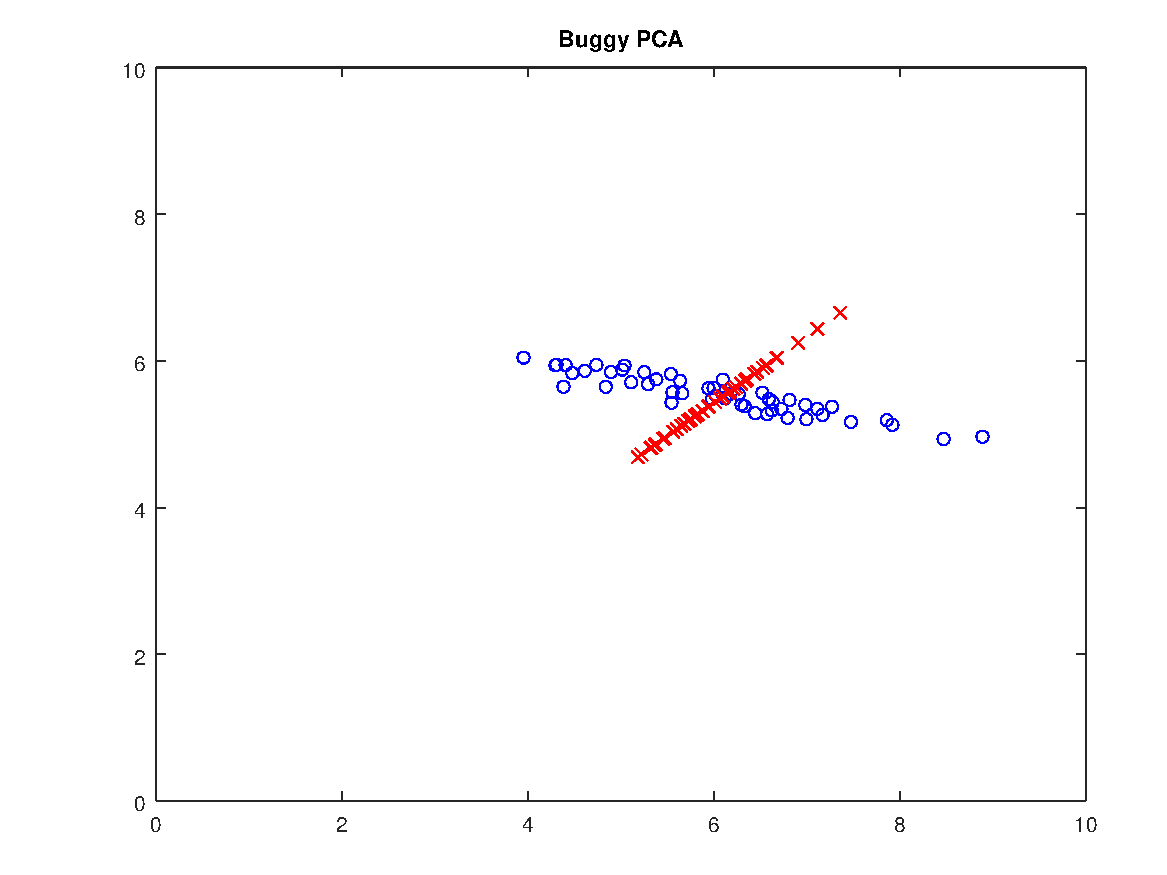
\includegraphics[width=3in]{buggy_pca-eps-converted-to.pdf} \hspace{0.4in}
\\

The blue circles are from the original dataset and the red crosses are the reconstructed points. \\

And this is how the reconstruction error may look like for Buggy PCA for the 2D dataset: 0.886903







\bibliographystyle{apalike}
\end{document}


